\documentclass[5p]{elsarticle} % seleccionar: preprint, review, 1p, 3p, 5p


\usepackage{mathtools}
\journal{ }


%to force all images and table in one single section
\usepackage{placeins}
% It is necesary to add \FloatBarrier in the text. 
% After that order, all the floating are shown.

%%%%%%%%%%%%%%%%%%%%%%%
%% Elsevier bibliography styles
%%%%%%%%%%%%%%%%%%%%%%%
%% To change the style, put a % in front of the second line of the current style and
%% remove the % from the second line of the style you would like to use.
%%%%%%%%%%%%%%%%%%%%%%%

%% Numbered
%\bibliographystyle{model1-num-names}

%% Numbered without titles
%\bibliographystyle{model1a-num-names}

%% Harvard
%\bibliographystyle{model2-names.bst}\biboptions{authoryear}

%% Vancouver numbered
%\usepackage{numcompress}\bibliographystyle{model3-num-names}

%% Vancouver name/year
%\usepackage{numcompress}\bibliographystyle{model4-names}\biboptions{authoryear}

%% APA style
%\bibliographystyle{model5-names}\biboptions{authoryear}

%% AMA style
%\usepackage{numcompress}\bibliographystyle{model6-num-names}

%% `Elsevier LaTeX' style
\bibliographystyle{elsarticle-num}

%%%%%%%%%%%%%%%%%%%%%%%
\hyphenation{}
\usepackage{eurosym}
\usepackage{threeparttable} % allow the use of footnote within tables

\usepackage{url}
\usepackage[colorlinks=true, citecolor=blue, linkcolor=blue, filecolor=blue,urlcolor=blue]{hyperref}

%to add the number to the lines
\usepackage{lineno}
\modulolinenumbers[5]

\usepackage{lineno,hyperref}
\modulolinenumbers[1]
\usepackage{amsmath}
\usepackage{siunitx}
\usepackage{eurosym}
\biboptions{numbers,sort&compress}
\usepackage[europeanresistors,americaninductors]{circuitikz}
\usepackage{adjustbox}
\usepackage{xspace}
\usepackage{caption}
\usepackage{booktabs}
\usepackage{tabularx}
\usepackage{threeparttable}
\usepackage{multicol}
\usepackage{float}
\usepackage{graphicx,dblfloatfix}
\usepackage{csvsimple}
%% new commands
\newcommand{\ubar}[1]{\text{\b{$#1$}}}
\newcommand*\OK{\ding{51}}
%\renewcommand*\nompostamble{\end{multicols}}
\newcommand{\specialcell}[2][c]{%
	\begin{tabular}[#1]{@{}l@{}}#2\end{tabular}}
\def\co{CO${}_2$}
\def\el{${}_{\textrm{el}}$}
\def\th{${}_{\textrm{th}}$}


%\renewcommand*{\today}{July, 10 2018}
%\hypersetup{draft} %to avoid problems with hyperref while drafting

\begin{document}

\begin{frontmatter}

\title{Early decarbonisation of the European energy system pays off}
\author[mymainaddress,iClimate]{Marta Victoria\corref{mycorrespondingauthor}}
\ead{mvp@eng.au.dk}
\author[mymainaddress]{Kun Zhu}
\author[kitaddress]{Tom Brown}
\author[mymainaddress,iClimate]{Gorm B. Andresen}
\author[mymainaddress,iClimate]{Martin Greiner}
\cortext[mycorrespondingauthor]{Corresponding author}
\address[mymainaddress]{Department of Engineering, Aarhus University, Inge Lehmanns Gade 10, 8000 Aarhus, Denmark}
\address[iClimate]{iCLIMATE Interdisciplinary Centre for Climate Change, Aarhus University}
\address[kitaddress]{Institute for Automation and Applied Informatics (IAI), Karlsruhe Institute of Technology (KIT), Forschungszentrum 449, 76344, Eggenstein-Leopoldshafen, Germany}


\begin{abstract}

In the context of increasing public climate change awareness and plummeting costs for wind and solar photovoltaics, discussions on increasing CO$_2$ reduction targets for Europe have started. Here, we model alternative transition paths with strict carbon budget for the sector-coupled networked European energy system. We show that up-to-date costs for wind and solar and the inclusion of highly resolved time series for balancing make climate action with renewables more cost-effective than previously seen. Ambitious CO$_2$ reductions in the short term not only trigger a cheaper transition but also incentivise more stable CO$_2$ prices and build rates for the required new capacities which could be beneficial from the point of view of investors, social acceptance, local economies, and jobs creation.

\end{abstract}

\begin{keyword}
myopic optimisation, carbon dioxide reduction, grid integration of renewable power, sector coupling, open energy modelling
%\texttt{elsarticle.cls}\sep \LaTeX\sep Elsevier \sep template
%\MSC[2010] 00-01\sep  99-00
\end{keyword}

\end{frontmatter}

\linenumbers

Achieving a climate-neutral European Union in 2050 \cite{in-depth_2018} requires meeting the milestones inbetween . Although carbon emissions will most likely sink by 20\% in 2020 relative to 1990 \cite{EEA_totalGHG}, it is unclear whether the 40\% objective settled for 2030 will be met. The national energy plans for the coming decade submitted by member states do not add up the necessary reduction to meet the target \cite{EU-appraisal_2019}, while in the context of a \textit{European Green Deal} a more ambitious reduction of 55\% is currently under discussion \cite{GreenDeal}. At the same time, led by young people \cite{Warren_2019}, society is advocating for more ambitious climate action. \\ %

A remaining global carbon budget of 800 Gigatons (Gt) of CO$_2$ can be emitted from 2018 onwards to limit the anthropogenic warming to 1.75$^{\circ}$C relative to the preindustrial period with a probability of more than 66\% \cite{IPCC_1.5}. Different sharing principles can be used to split the global carbon budget into regions and countries \cite{Raupach_2014}. Considering an equal per-capita distribution translates into a quota of 48 GtCO$_2$ for Europe. An approach that took into account historical emissions would lead to more ambitious targets for Europe than other regions \cite{Matthews_2016}. Assuming that sectoral distribution of emissions within Europe remains at present values, the carbon budget for the generation of electricity and provision of heating in the residential and services sectors accounts for approximately 21 GtCO$_2$, \cite{UNFCCC_inventory} and Supplementary Note 2. The budget increases to 33 GtCO$_2$ when the transport sector is included. \\ 

\begin{figure}[!h]
\centering
	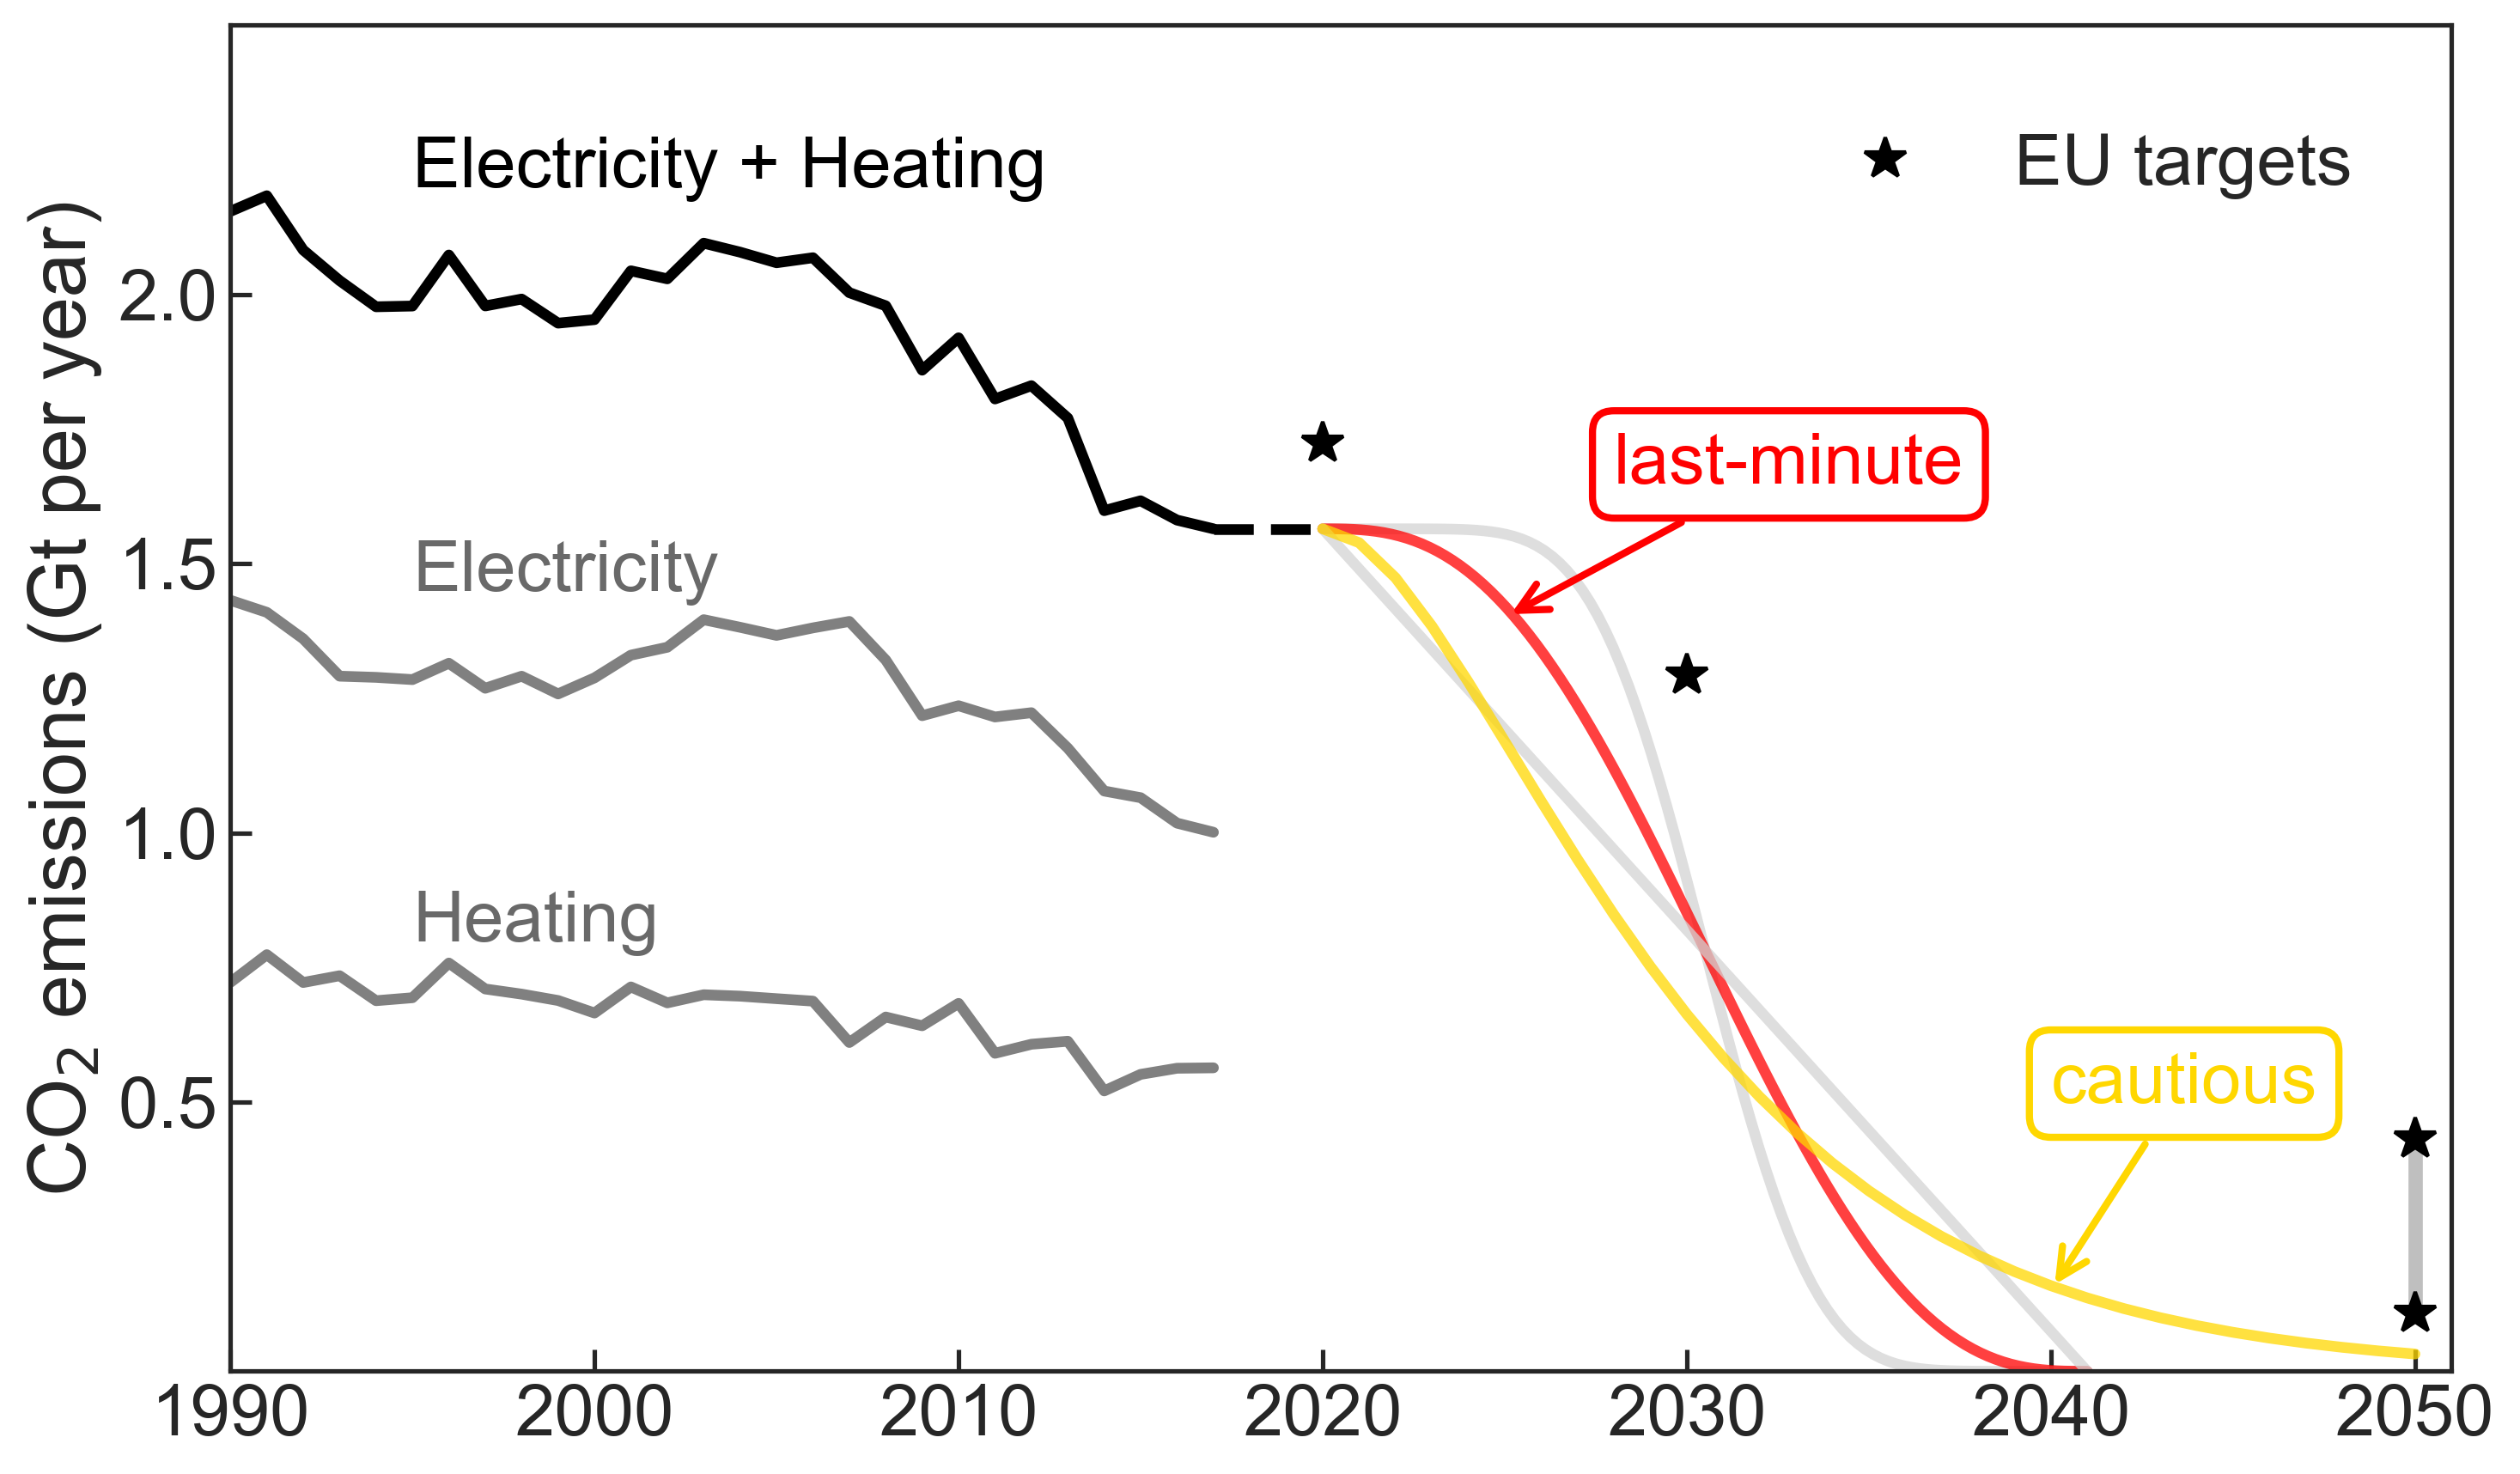
\includegraphics[width=\columnwidth]{../figures/carbon_budget.png}
\caption{Historical CO$_2$ emissions from the European power system and heating supply in the residential and services sectors \cite{UNFCCC_inventory}. The various future transition paths shown in the figure have the same cumulative CO$_2$ emissions, which correspond to the remaining 21 Gt CO$_2$ budget to avoid human-induced warming above 1.75$^{\circ}$C with a probability of greater than 66\%, assuming current sectoral distribution for Europe, and equity sharing principle among regions. Black stars indicate committed EU reduction targets, while white stars mark targets under discussion.} \label{fig_carbon_budget} 
\end{figure}

In this work, we use an hourly-resolved sector-coupled networked model of the European energy system and myopic optimisation in 5-years steps from 2020 to 2050 to investigate the impact of different CO$_2$ reduction paths with the same carbon budget. In every time step, the expansion of generation, storage and interconnection capacities in every country is allowed if it is cost-effective under the corresponding global emissions constraint. We show that up-to-date costs for wind and solar that take into account recent capacity additions and technological learning make climate action with renewables more cost-effective than previously seen. Furthermore, we find that a transition path with more ambitious short-term CO$_2$ targets reduces the cumulative system cost and requires a smoother increase of the CO$_2$ price and more stable build rates. Our research includes the coupling  with heating and transport sectors, which is absent in transition path analyses for the European power system \cite{Plesmann_2017, Gerbaulet_2019, Poncelet_2016}, as well as up-to-date cost assumption for wind and solar PV together with hourly resolution, in contrast to the outdated cost and low temporal resolution in Integrated Assessment Models (IAMs) \cite{Creutzig_2017, Krey_2019}. We use an open model, which ensures transparency and reproducibility of the results \cite{Pfenninger_2017, Pfenninger_2018}.

\FloatBarrier

\paragraph{\textbf{Myopic optimisation with sector coupling}} \

Electricity generation is expected to spearhead the transition spurred by the dramatic cost reduction of wind energy \cite{Lantz_2012} and solar photovoltaics (PV) \cite{Creutzig_2017, Haegel_2019}. A vast body of literature shows that a power system based on wind, solar, and hydro generation can supply hourly electricity demand in Europe as long as proper balancing is provided \cite{Eriksen_2017, Schlachtberger_2017, Gils_2017a, Brown_response}. This can be done by reinforcing interconnections among neighbouring countries \cite{Rodriguez_2014} to smooth renewable fluctuations by regional aggregation or through temporal balancing using local storage \cite{Rasmussen_2012, Cebulla_2017, Victoria_2019_storage}. Moreover, coupling the power system with other sectors such as heating or transport could provide additional flexibilities facilitating the system operation and simultaneously helping to abate emissions in those sectors \cite{Connolly_2016, Brown_2018, Child_2019}. \\

CO$_2$ emissions from heating in the residential and services sectors show a more modest historical reduction trend compared to electricity generation (Fig. \ref{fig_carbon_budget}). Nordic countries have been particularly successful in reducing carbon emissions from the heating sector by using sector-coupling strategies, Supplementary Note 3. Denmark, where more than half of the households are connected to district heating systems \cite{Gross_2019}, has shifted the fuel used in Central Heat and Power (CHP) units from coal to biomass and urban waste incineration \cite{DEA_2015}. Sweden encouraged a large-scale switch from electric resistance heaters to heat pumps \cite{Gross_2019} and it is now supported by high CO$_2$ prices \cite{Carbon_pricing_2019} and low electricity taxes.\\ 

Greenfield optimisation of the future European energy system, that is, building the system from scratch, shows that sector-coupling decreases the system cost and reduces the need for extending transmission lines due to the additional local flexibility brought by the heating and transport sectors \cite{Brown_2018}. Sector-coupling allows large CO$_2$ reductions before large capacities of storage become necessary, providing more time to further develop storage technologies \cite{Victoria_2019_storage}. Greenfield optimisation is useful to investigate the optimal configuration of the fully-decarbonised system, but it does not provide insights on how to transition towards it. Today's generation fleet and decisions taken in intermediate steps will shape the final configuration. Transition paths for the European power system have been analysed using myopic optimisation, without full foresight over the investment horizon \cite{Bogdanov_2019, Plesmann_2017, Gerbaulet_2019, Poncelet_2016}. Myopic optimisation results in higher cumulative system cost than optimising the entire transition period with perfect foresight because the former leads to stranded investments \cite{Gerbaulet_2019, Heuberger_2018}. However, the myopic approach is less sensitive to the assumed discount rate and can capture better short-sighted behaviour of political actors and investors \cite{Poncelet_2016, Gerbaulet_2019}. 

\paragraph{\textbf{Alternative transition paths}} \


Here, we investigate the consequences of following two alternative transition paths. The Gentle path represents a cautious approach in which significant emissions reductions are attained in the early years. In the Sudden path, the low initial reduction targets quickly deplete the carbon budget, requiring a sharp reduction later. As in Aesop's fable ``The Tortoise and the Hare'', 
the tortoise wins the race by making steady progress, whereas following the hare and delaying climate action requires a late acceleration that will be more expensive and might be unfeasible. 

\paragraph{\textbf{Cumulative costs}} The two alternative paths arrive at a similar system configuration in 2050, Fig. \ref{fig_system_cost}. Towards the end of the period, under heavy CO$_2$ restriction, balancing technologies appear in the system. They include large storage capacities comprising electric batteries and hydrogen storage, and production of synthetic methane.  Cumulative system cost for the Gentle path represents 6,994 billion euros (B\EUR), while the Sudden path accounts for 7,341 B\EUR. The newly built conventional capacity for electricity generation is very modest in both cases, Fig. \ref{fig_age_distribution} and Supplementary Note 8. No new lignite, coal or nuclear capacity is installed. Thus, at the end of both paths, conventional technologies include only gas-fueled power plants, CHP and boilers. Biomass contributes to balancing renewable power but plays a minor role. Decarbonising the power system has proven to be cheaper than the heating sector \cite{Zhu_2019}. Consequently, although CO$_2$ allowances differ, the electricity sector gets quickly decarbonised in both paths and more notable differences appear in new conventional heating capacities, Fig. \ref{fig_heating_expansion}. Under the tortoise strategy yearly costs initially decrease as the power system takes advantage of the low costs of wind and solar. Removing the final emissions in heating causes total costs to rise again towards 2050.

\begin{figure*}[!h]
\centering
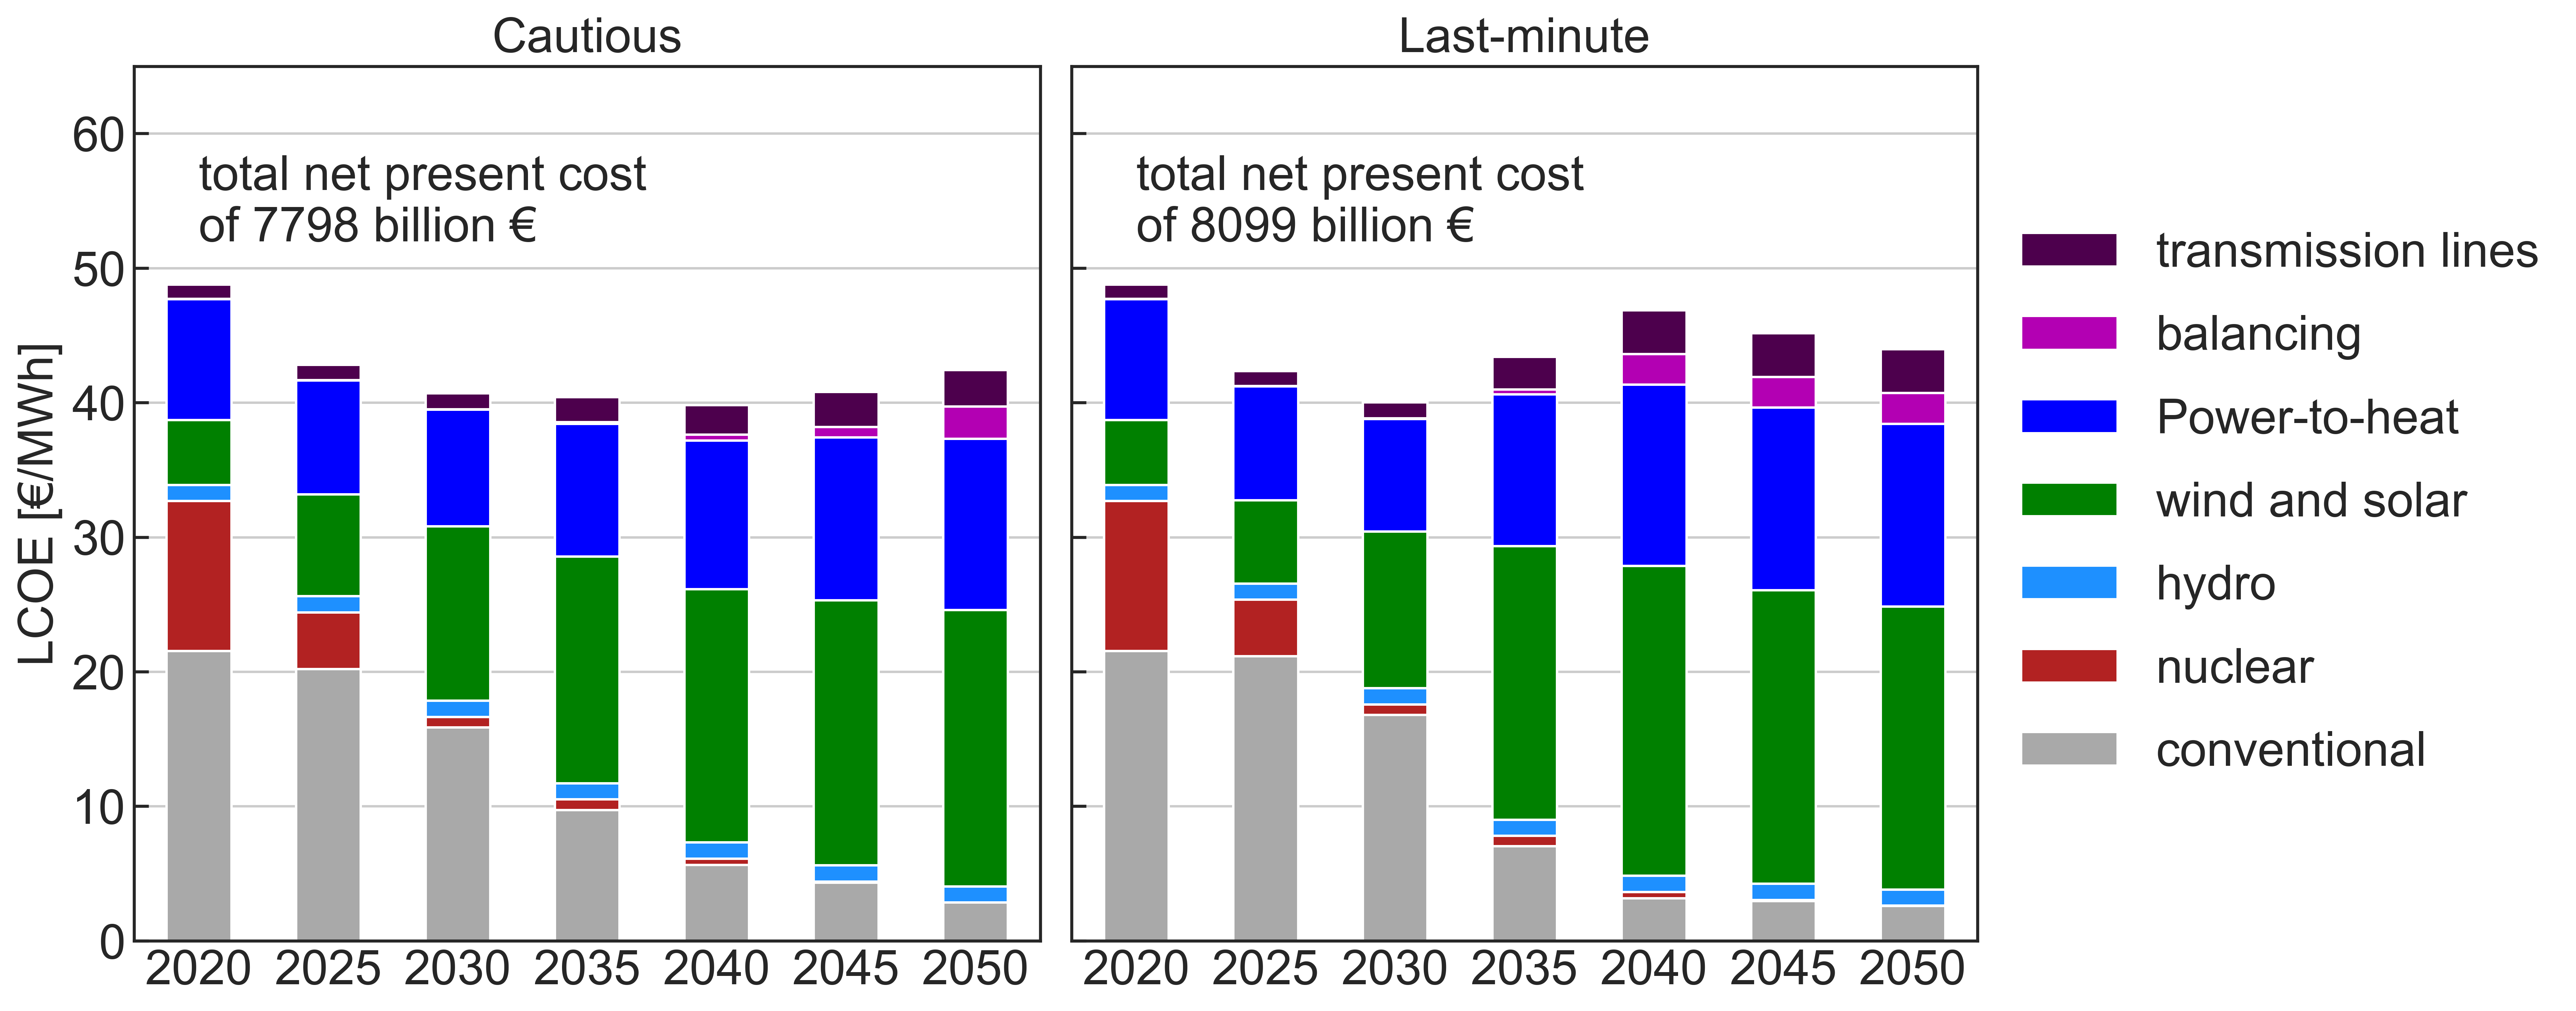
\includegraphics[width=0.9\textwidth]{../figures/LCOE_Base.png}
\caption{Levelized Cost of Energy (LCOE) for the European electricity and heating system throughout transition paths Gentle and Sudden shown in Fig. \ref{fig_carbon_budget}. Conventional includes costs associated with coal, lignite, and gas power plants producing electricity as well as costs for fossil-fueled boilers and CHP units. Power-to-heat includes costs associated with heat pumps and heat resistors. Balancing includes costs of electric batteries, H$_2$ storage, and methanation.} \label{fig_system_cost} 
\end{figure*}

\begin{figure*}[!h]
\centering
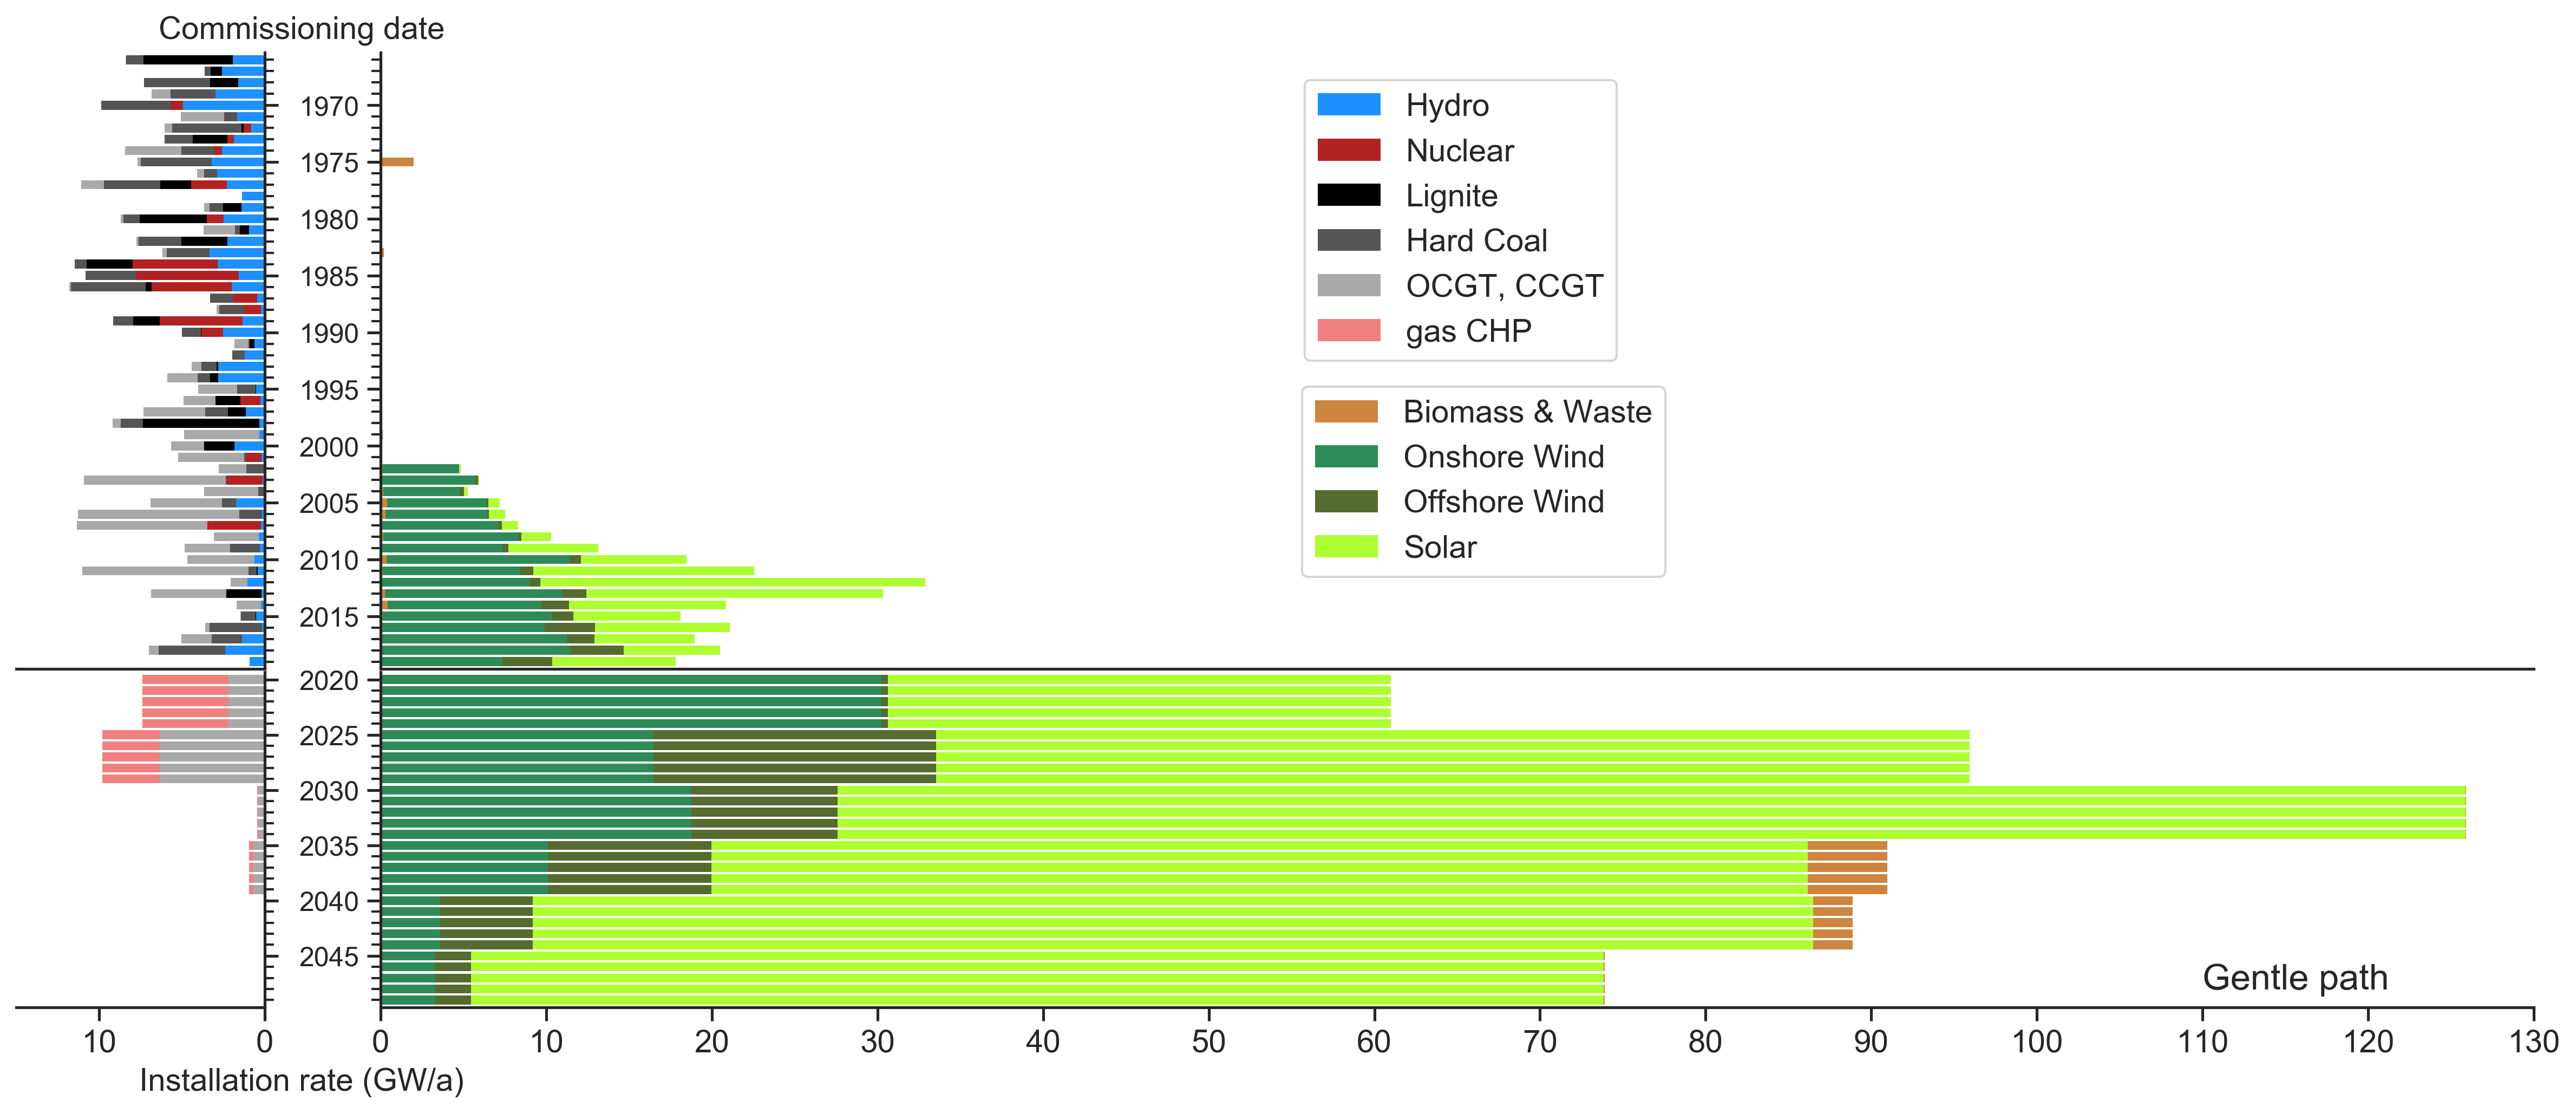
\includegraphics[width=\textwidth]{../figures/age_distribution_Base_Gentle.png}
\caption{Age distribution of European power plants in operation \cite{powerplantmatching, IRENA_2019} and required annual installation throughout the Gentle path.} \label{fig_age_distribution} 
\end{figure*}

\paragraph{\textbf{Stranded assets}} Part of the existing conventional capacities become stranded assets, in particular, coal, lignite, CCGT (which was heavily deployed in the early 2000s, Fig. \ref{fig_age_distribution}) and gas boilers. As renewable capacities deploy, utilisation factors for conventional power plants decline and they do not recover their total expenditure via market revenues, Supplementary Note 8. Up to 2035, operational expenditure for gas-fueled technologies are lower than market revenues so they are expected to remain in operation. Unexpectedly, the sum of expenditures not recovered via market revenues is similar for both paths. In the Sudden path, high CO$_2$ prices justify producing up to 220 TWh/a of synthetic methane in 2040. This enables CCGT and gas boilers to keep operating allowing them to recover part of their capital expenditure, but the consequence is a higher cumulative system cost, as previously discussed. Although closing plants early might be seen as an unnecessary contribution to a higher cost of energy, it must be remarked that the early retirement of electricity infrastructure has been identified as one of the most cost-effective actions to reduce committed emissions and enable a 2$^{\circ}$C-compatible future evolution of global emissions \cite{Tong_2019}.


\paragraph{\textbf{Transition smoothness}} A timely transition is challenging yet feasible given historic build rates. Decarbonising the electricity and heating sectors using wind and solar PV requires 
duplicating the highest historical build rates seen in individual countries, Fig. \ref{fig_age_distribution} and Supplementary Note 4. Consequently, attaining higher build rates to also decarbonise transport and industry sectors seems feasible. Wind and solar PV supply most of the electricity demand in 2050, complemented by hydro and with a minor biomass contribution. Previously, most IAMs have emphasized the importance of bioenergy or carbon capture and storage and failed to identify the key role of solar PV due to their unrealistically high cost assumptions for this technology, see \cite{Creutzig_2017, Krey_2019} and Supplementary Note 7.2. \\

\begin{figure}[!h]
\centering
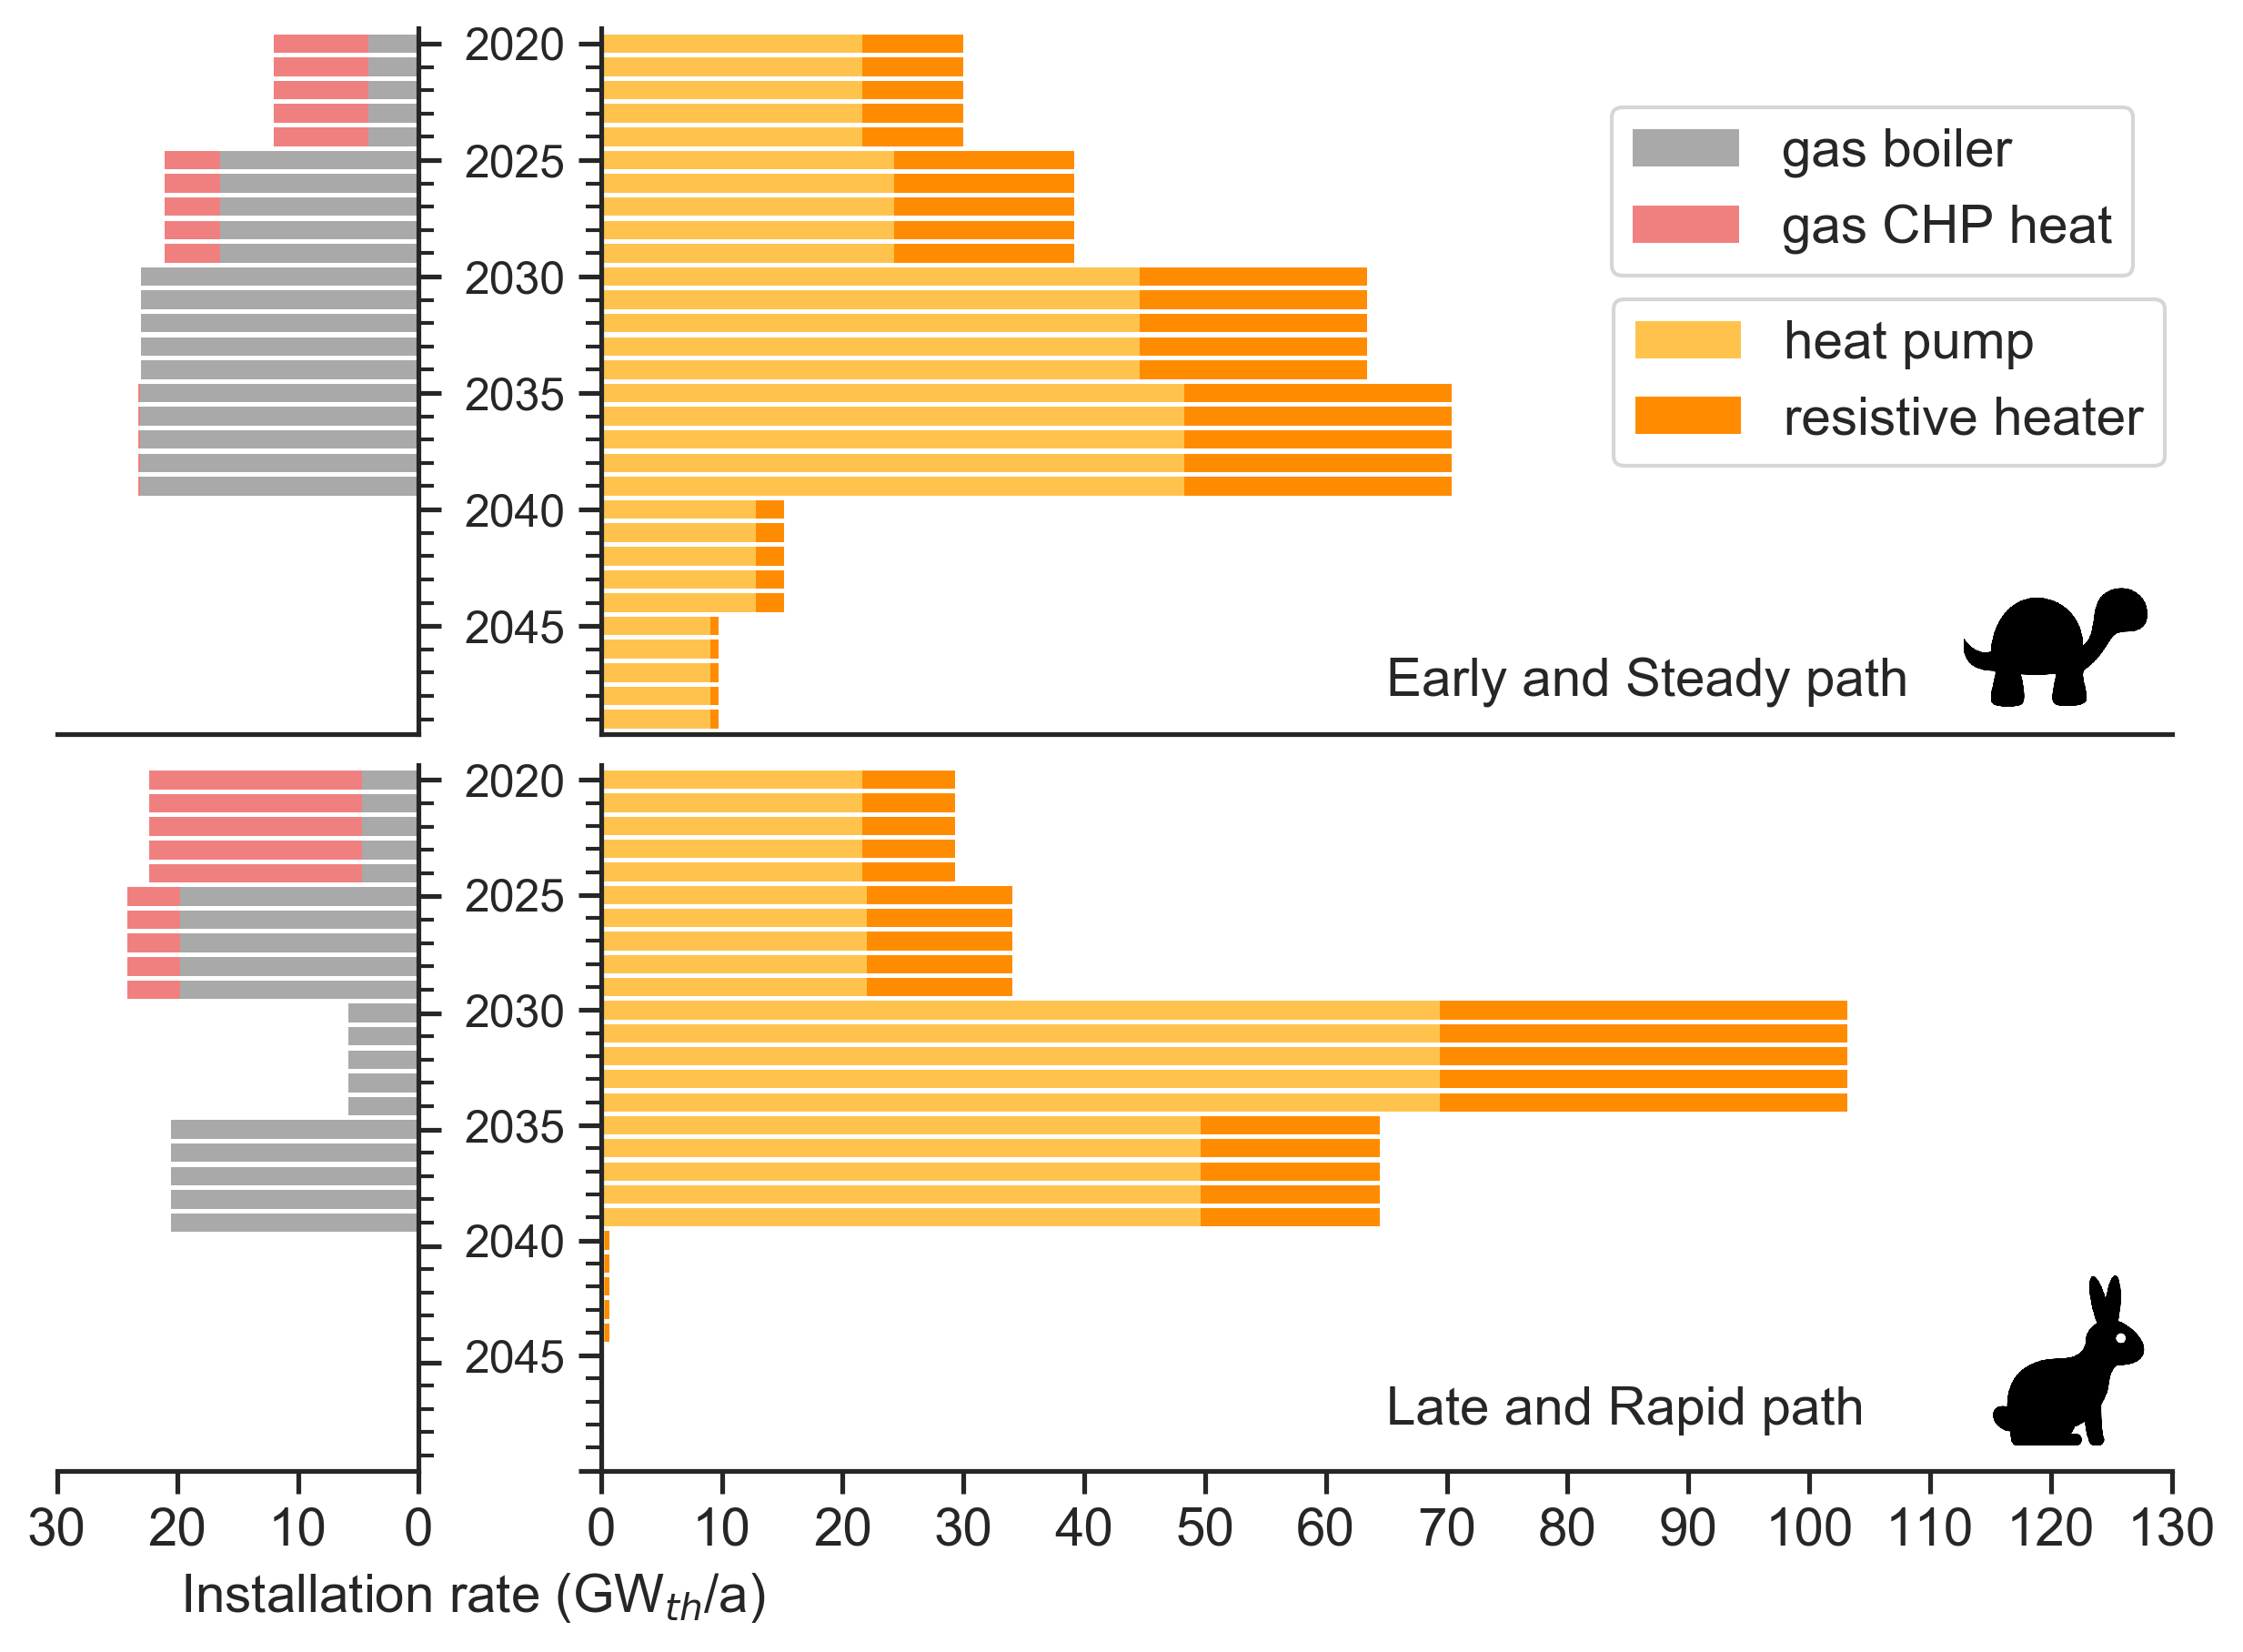
\includegraphics[width=\columnwidth]{../figures/heating_expansion_Base.png}
\caption{Required expansion of heating capacities in both paths. Maximum heating capacities are shown for CHP plants.} \label{fig_heating_expansion} 
\end{figure}

During the past decade, several European countries have shown sudden increments in the annual build rate for solar PV, followed by equivalent decrements one or two years later. Italy, Germany, UK, and Spain show clear peaks (Supplementary Note 4)  due to the combination of a fast cost decrease of the technology and unstable regulatory frameworks whose details are country-specific. These peaks are lethal for local businesses. The sudden shrinkage of annual build capacity results in companies bankruptcy and lost jobs. The Gentle path requires a smoother evolution of build rates which could better accommodate the cultural, political, and social aspects of the transition \cite{Geels_2017}. The mild evolution could also facilitate reaching a stationary situation in which build rates offset decommissioning. \\ 

CO$_2$ prices much higher than those historically attained in the ETS market are necessary at the end of the transition, Fig. \ref{fig_co2price}. The Gentle path requires a smoother evolution of CO$_2$ price, which will be preferred by investors. CO$_2$ price is only an indicator of the price gap between polluting and clean technologies and several policies can be established to fill that gap. Among others, sector-specific CO$_2$ taxes \cite{Carbon_pricing_2019}, direct support for renewables that reduce investor risk, and consequently the cost of capital and LCOE of the technology \cite{Vartiainen_2019}, or regulatory frameworks that incentivise the required technologies such those promoting rooftop PV installations or ensuring the competitiveness of district heating systems. 

\begin{figure}[!h]
\centering
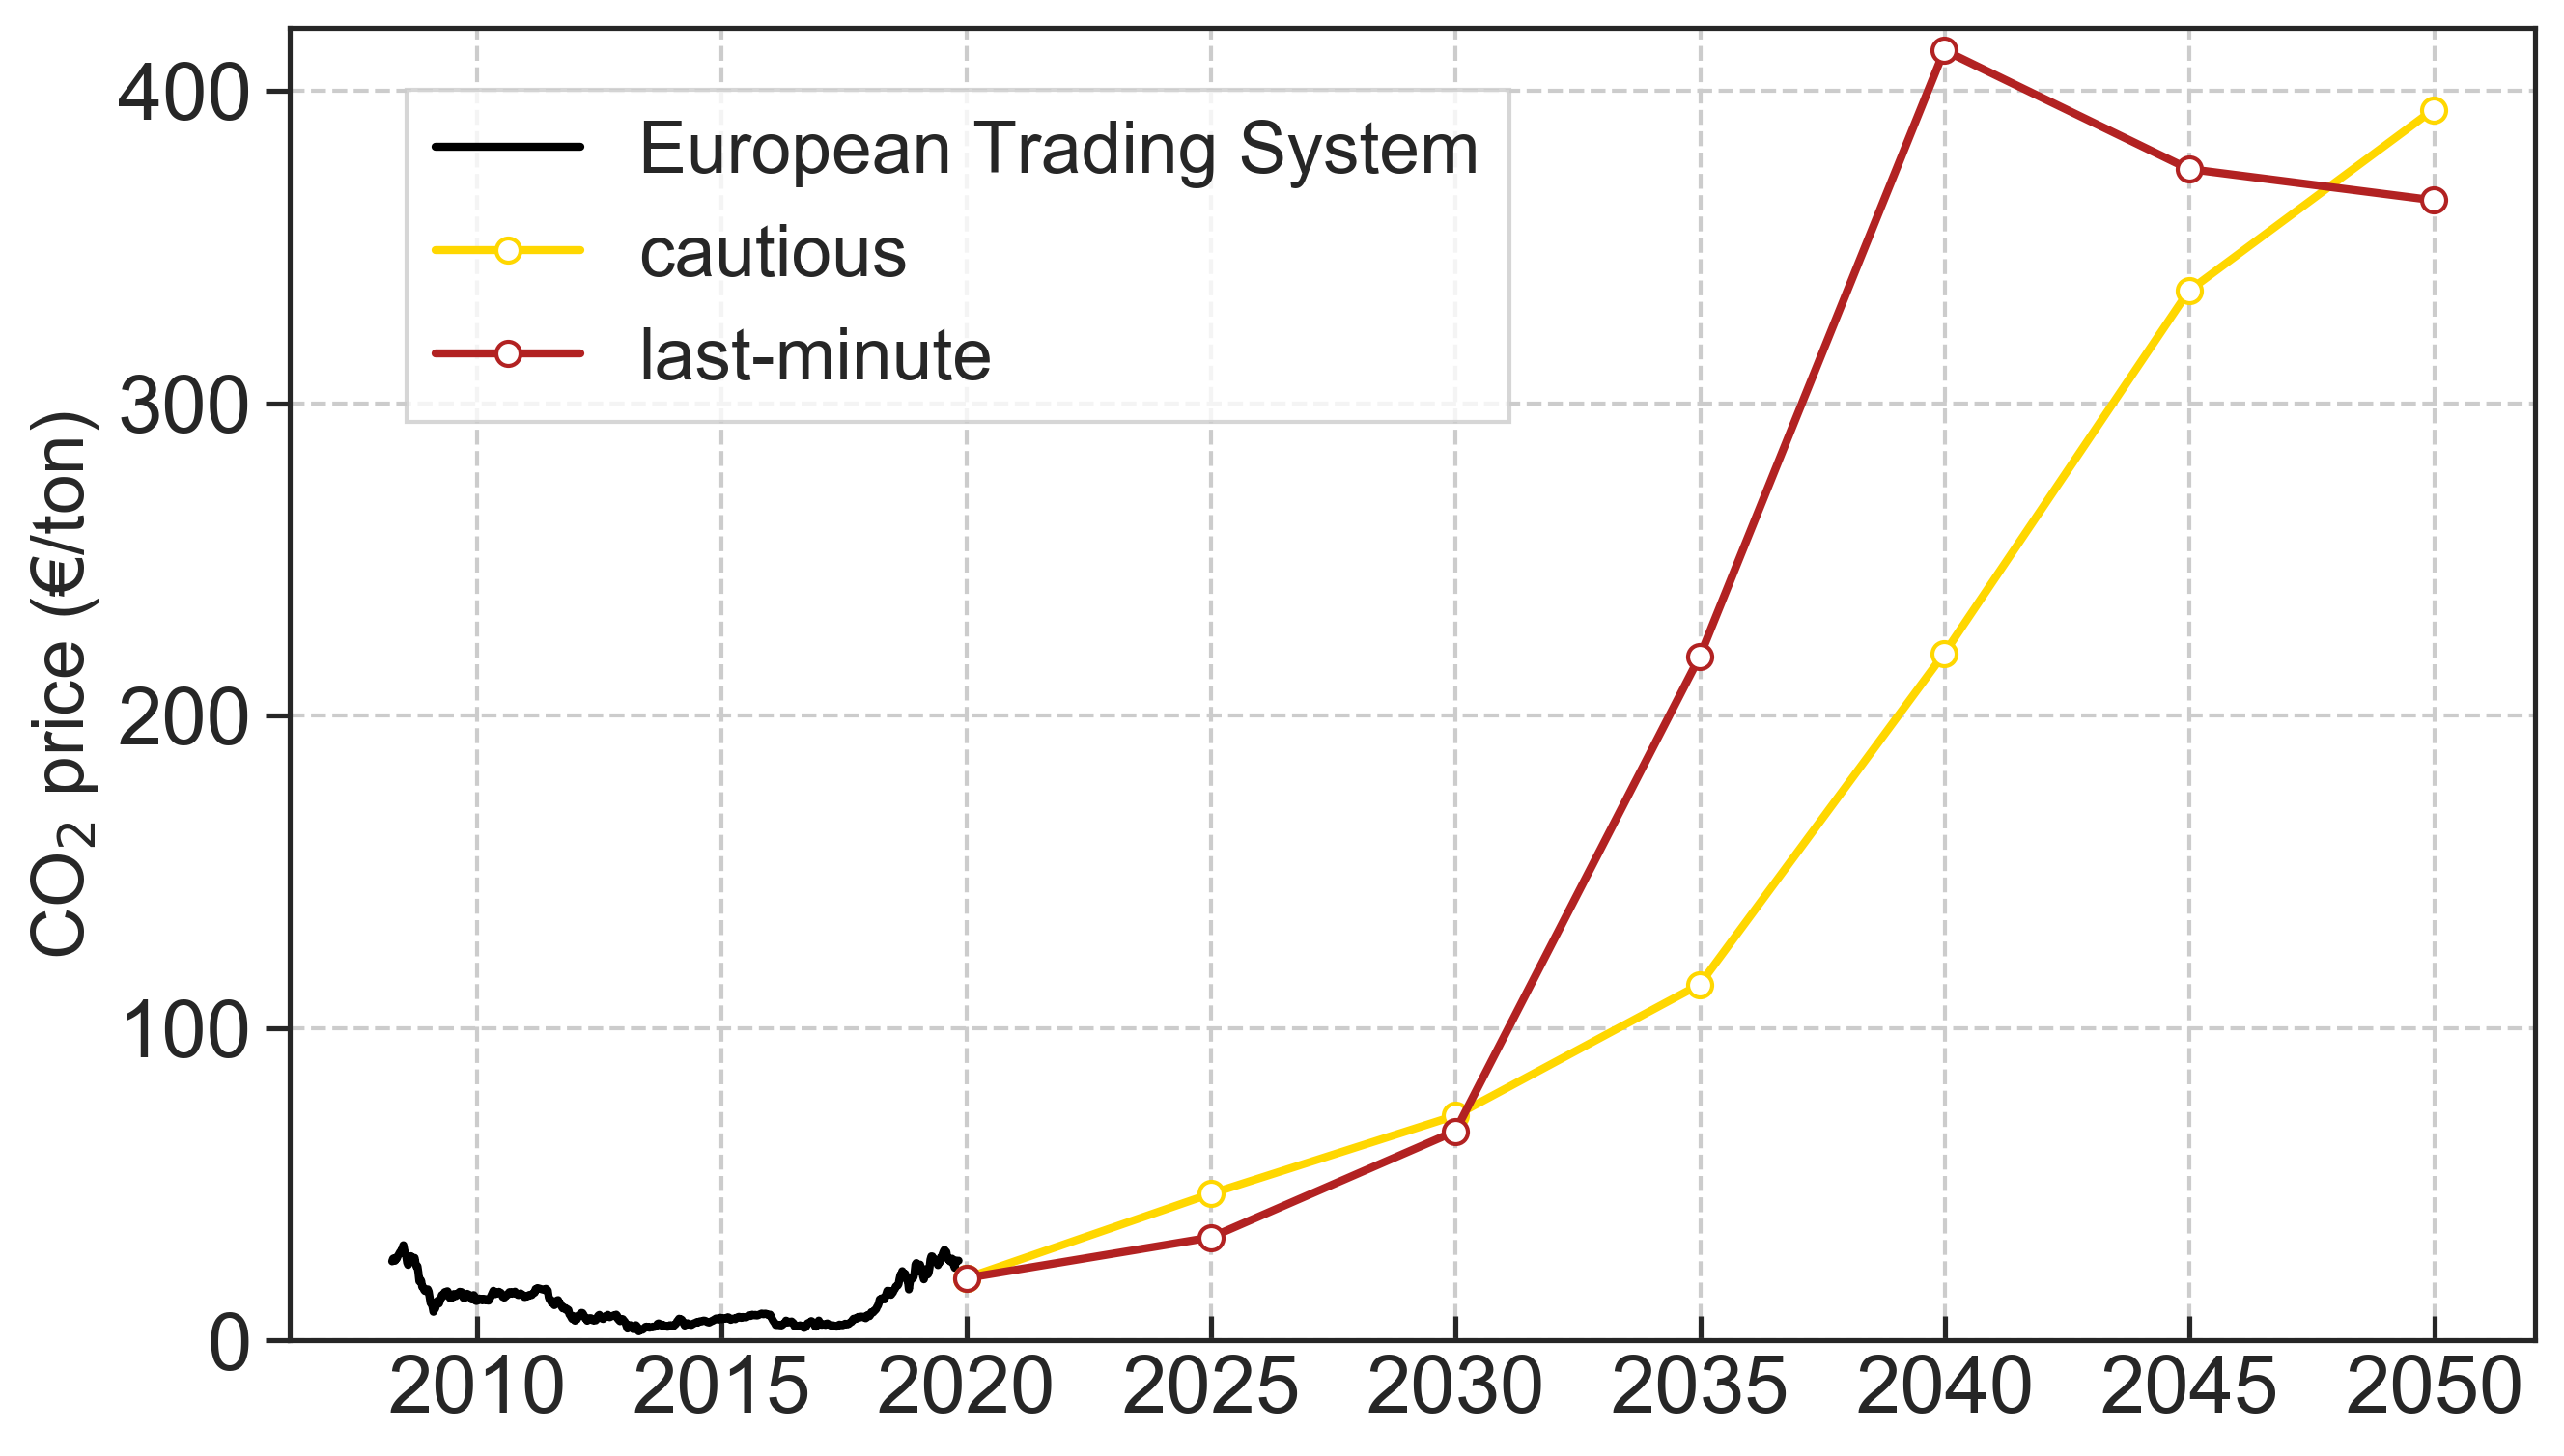
\includegraphics[width=\columnwidth]{../figures/co2_price.png}
\caption{Historical evolution of CO$_2$ price in the EU Emissions Trading System \cite{ETS} and required CO$_2$ price obtained from the model throughout transition paths shown in Fig. \ref{fig_carbon_budget}. 
Co-benefits of reducing CO$_2$ emissions in Europe due to avoided premature mortality, reduced lost workdays, and increased crop yields are estimated in the range of 125-425 \EUR/ton CO$_2$ \cite{Vandyck_2018}.} \label{fig_co2price} 
\end{figure}

\paragraph{\textbf{Hourly and country resolved results}} \

At every time step, the optimal renewable mix in every country depends on the local resources and the already existing capacities, see Supplementary Note 8.2. Nevertheless, the analysis of near-optimal solutions has recently shown that country-specific mixes can vary significantly while keeping the total system cost only slightly higher than the minimum \cite{Neumann_2019}. \\

Modelling an entire year with hourly resolution unveils the strong links between renewable generation technologies and balancing strategies. For countries and years in which large solar PV capacities are deployed, it is also cost-effective to install large battery capacities to smooth the strong daily solar generation pattern. Conversely, onshore and offshore wind capacities require hydrogen storage and reinforced interconnections to balance wind synoptic fluctuations \cite{Rasmussen_2012, Schlachtberger_2017, Victoria_2019_storage}. %The strong bounds existing between solar PV-battery and wind-hydrogen  
This can also be appreciated by looking at the dominant dispatch frequencies exposed by the Fourier power spectra of the Europe-aggregated time series in 2050 on the Gentle path, Fig. \ref{fig_Fourier}. \\

\begin{figure}[!h]
\centering
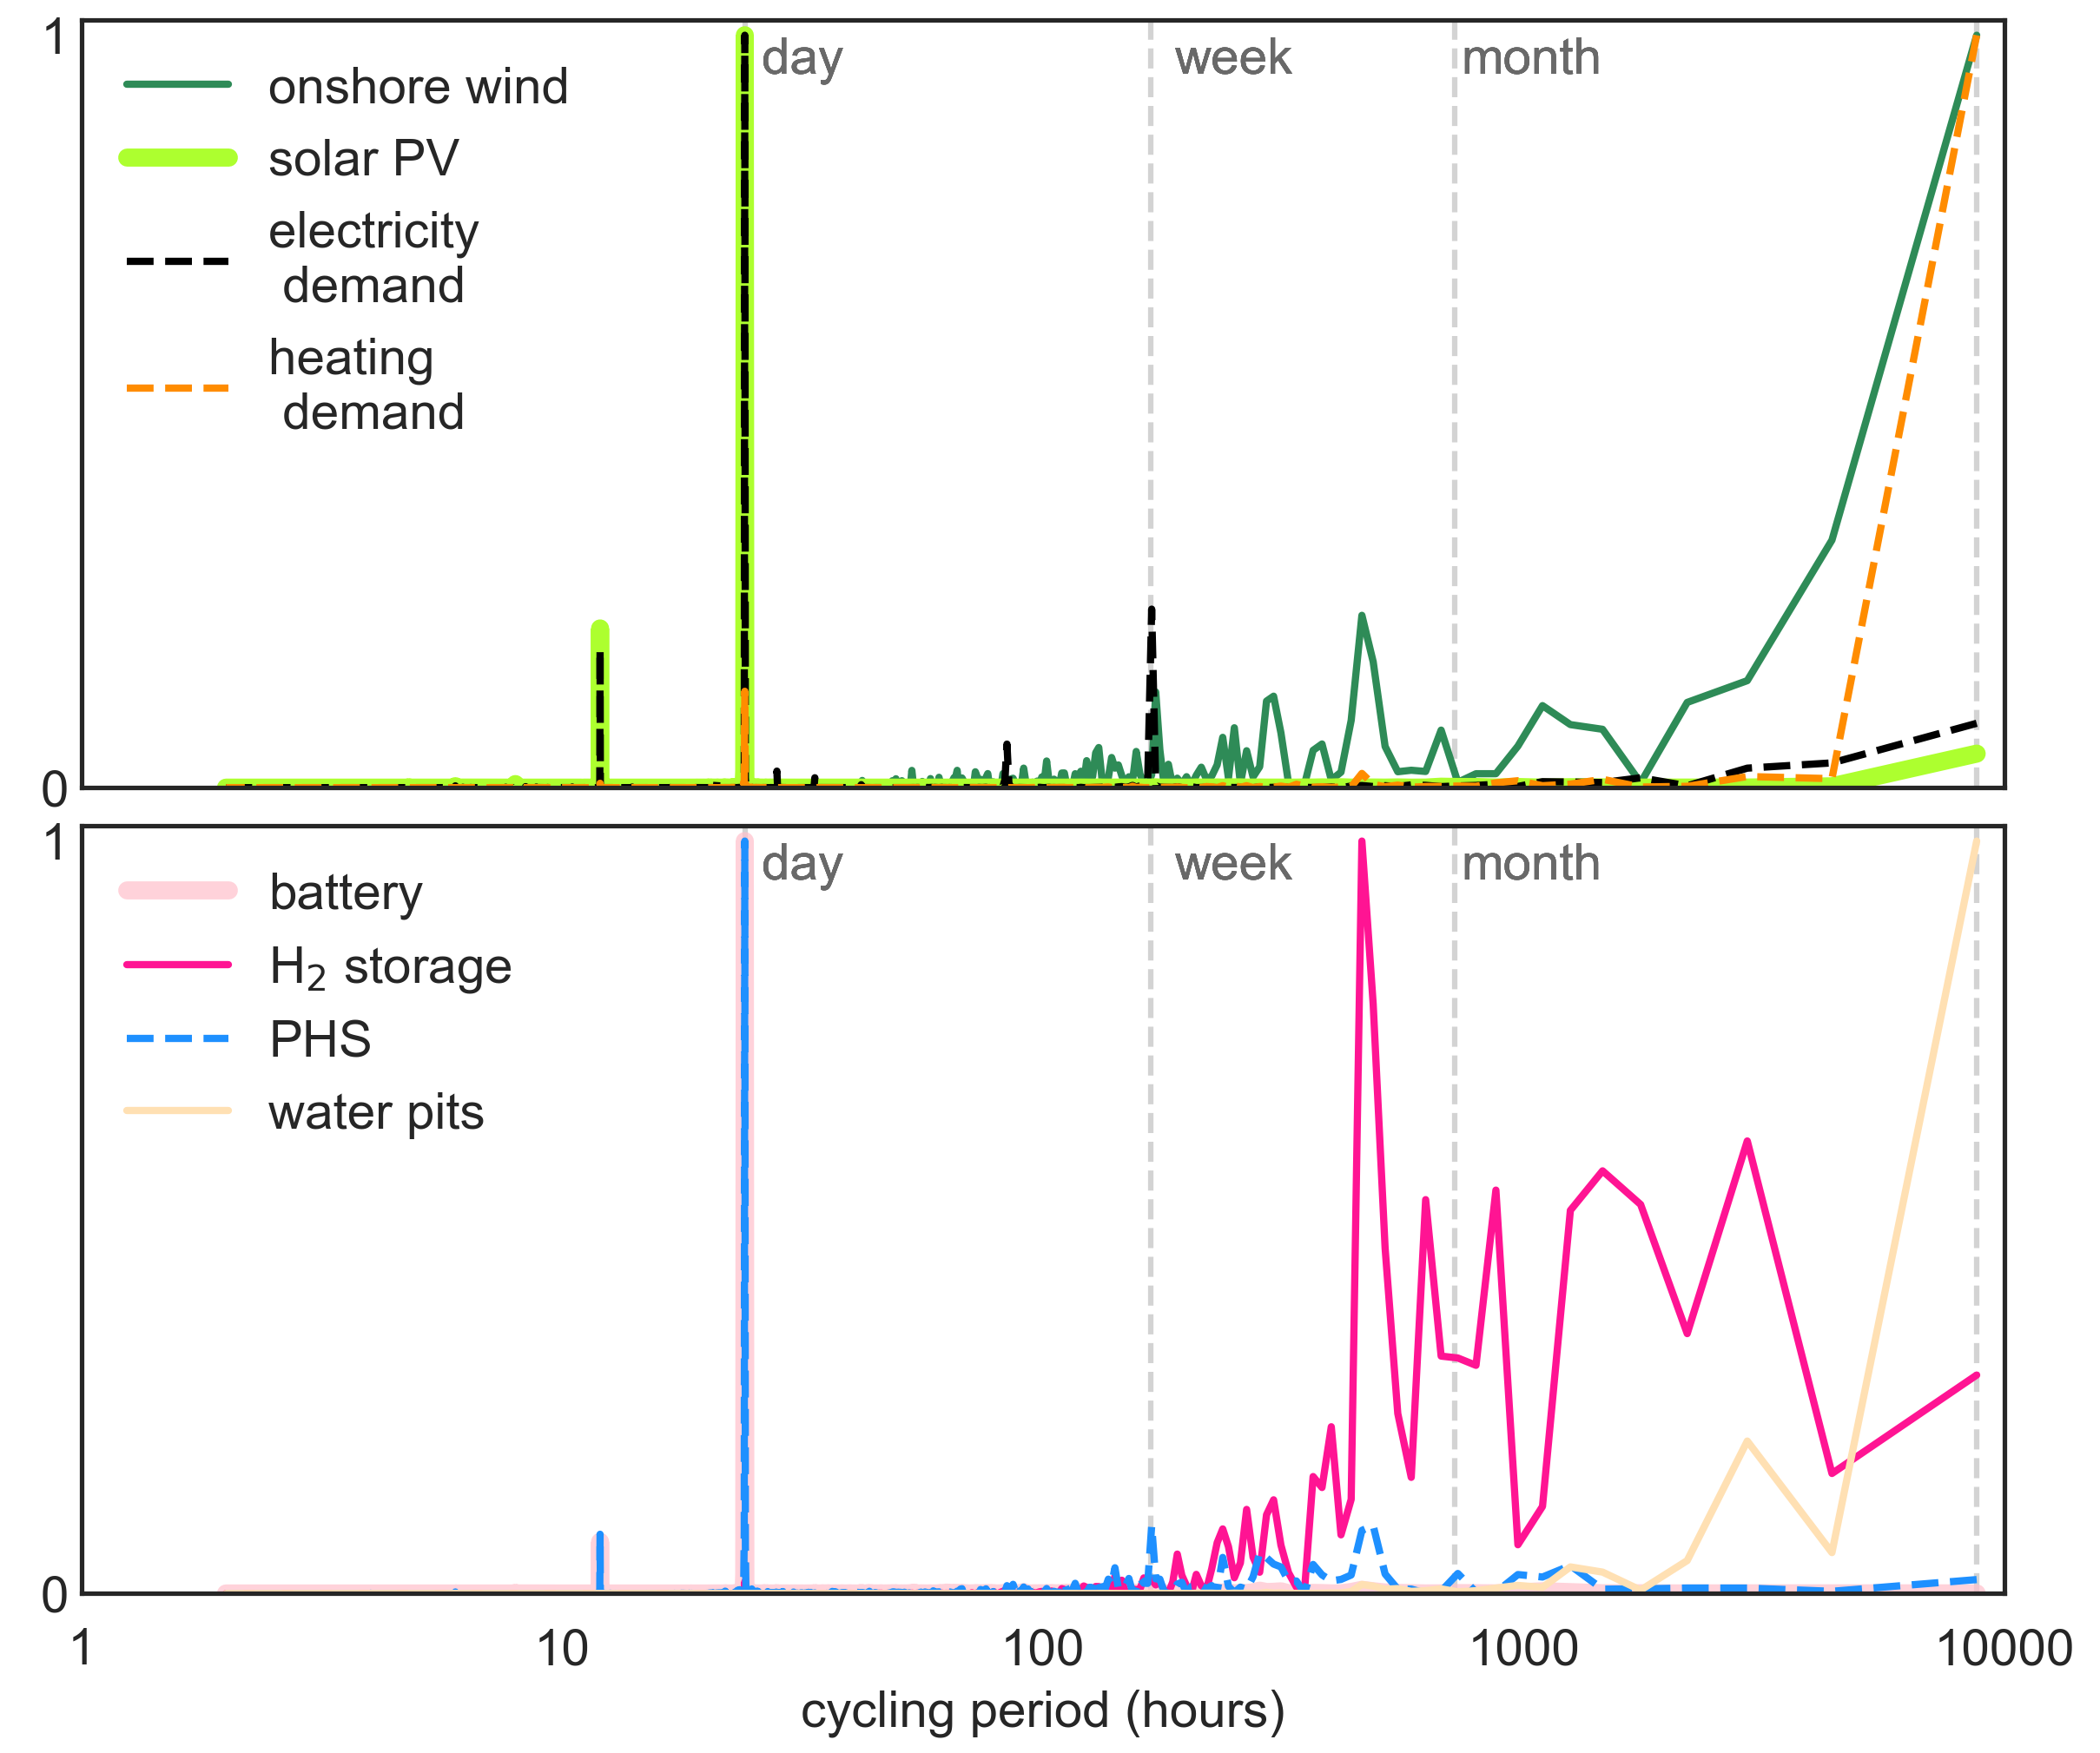
\includegraphics[width=\columnwidth]{../figures/Fourier.png}
\caption{Fourier power spectra of wind and solar PV generation, electricity and heating demand, as well as storage technologies dispatch. Time series represent the Europe-aggregated generation/demand for the Gentle path in 2050.} \label{fig_Fourier} 
\end{figure}

IAMs with similar spatial resolution have also been used to investigate the sector-coupled decarbonisation of Europe \cite{in-depth_2018, JRC-EU-TIMES, Creutzig_2017}. However, IAMs typically use a much lower time resolution, \textit{e.g.}, using a few time slices to represent a full year \cite{JRC-EU-TIMES, Loffler_2019, Poncelet_2016, McGlade_2015, Babrowski_2014} or considering the residual load duration curve \cite{Creutzig_2017, Ueckerdt_2017}, and some IAM assume very high integration costs for renewables \cite{Pietzcker_2014}. The hourly resolution in our model reveals several effects that are critical to the operation of highly renewable systems, such as the variable, but correlated solar and wind power generation smoothed by the grid, the role of long-term storage, and the system operation during cold spells, \textsl{i.e.}, a cold week with low wind and solar generation.

%\FloatBarrier
 
\paragraph{\textbf{Results robust under different scenarios}} \

District heating (DH) has proven to be extremely useful to decarbonise the heating sector. It allows cheaper central technologies such as heat pumps and CHP units, enables a faster conversion because it is easier to substitute one central heating unit than a myriad of individual domestic systems, and facilitates long-term thermal energy storage, via cheap large water pits, Fig.\ref{fig_Fourier}, that help to balance the large seasonal variation of heating demand, Supplementary Note 6. So far, we have assumed that DH penetration remains constant at 2015 values. When DH is assumed to expand linearly so that in 2050 it supplies the entire urban heating demand in every country, cumulative system cost for the Gentle path reduces by 238 B\EUR. This roughly offsets the cost of extending and maintaining the DH networks and avoids the additional expansion of gas distribution networks. When a 2\% reduction of space heating demand per year is assumed due to renovations of the building stock, cumulative system cost decreases by 760 B\EUR compared to paths with constant heating demand, significantly offsetting costs of renovations. When the model is allowed to optimise transmission capacities after 2030, together with the generation and storage assets, the optimal configuration at the end of the paths includes a transmission volume approximately three times higher than that of 2030. Although the cumulative system cost is 93 B\EUR lower, it is unclear to what extent it compensates the social acceptance issues associated with extending transmission capacities. Neither of the paths install new nuclear capacity. This technology is only part of the optimal system in 2050 when nuclear costs are lower by 15\% compared to the reference cost and no transmission capacity expansion is allowed. In all the previous scenarios, the difference in cumulative system cost for the Gentle and Sudden path is roughly the same.

\paragraph{\textbf{Transport}} \

Finally, Gentle and Sudden paths are re-run including the coupling of road and rail transport, as described in Supplementary Note 6.5. For every time step, the electrification of transport is assumed to be equal to the CO$_2$ emissions reduction relative to 2020. In this way, emissions in that sector sink roughly parallel to those of heating and electricity sectors. The extra electricity demand raises cumulative system cost, but the LCOE remains similar throughout the transition. The additional flexibility provided by EVs reduces the need for static batteries and incentivises a higher solar PV penetration, as previously observed \cite{Brown_2018, Victoria_2019_storage}.

\paragraph{\textbf{Conclusions}} \

When comparing alternative transition paths for the European energy system with the same carbon budget, we find that those including a gentle CO$_2$ reduction are consistently around 300 B\EUR cheaper than those paths where low targets in the initial period demand a sharper reduction later.  We found that up-to-date costs for wind and the inclusion of highly resolved time series for balancing make climate action with renewables more cost-effective than previously seen. The required renewable build rates to decarbonise the electricity and heating sectors correspond to the highest historical country-level values, making the transition challenging yet feasible. We have shown that early action not only allows room for decision-making later but it is also pays off.  



\FloatBarrier
\section{Methods}

The system configuration is optimised by minimising annualised system cost in every time step (one every 5 years), under the global CO$_2$ emissions cap imposed by the transition path under analysis (Fig. \ref{fig_carbon_budget}). This can be considered a myopic approach since the optimisation has no information about the future. The cumulative CO$_2$ emissions for the Gentle and Sudden transition paths is equal to a carbon budget of 21 GtCO$_2$. In every time step, generation, storage, and transmission capacities in every country are optimised assuming perfect competition and foresight as well as long-term market equilibrium. Besides the global CO$_2$ emission cap, other constraints such as the demand-supply balance in every node, and the maximum power flowing through the links are imposed to ensure the feasibility of the solution, Supplementary Note 5. \

We use a one-node-per-country network, including 30 countries corresponding to the 28 European Union member states as of 2018 excluding Malta and Cyprus but including Norway, Switzerland, Bosnia-Herzegovina, and Serbia (Fig. 18 in Supplementary Note 8). Countries are connected by High Voltage Direct Current (HVDC) links whose capacities can be expanded if it is cost-effective. In the power sector, electricity can be supplied by onshore and offshore wind, solar photovoltaics (PV), hydroelectricity, Open Cycle Gas Turbines (OCGT), Combined Cycle Gas Turbines (CCGT), Coal, Lignite, and Nuclear power plants, and Combined Heat and Power (CHP) units using gas, coal or biomass. Electricity can be stored using Pumped Hydro Storage (PHS), static electric batteries, and hydrogen storage. Hydrogen is produced via electrolysers and converted back into electricity using fuel cells. Methane can be produced by combining Direct Air Captured (DAC) CO$_2$ and electrolysed-H$_2$ in the Sabatier reaction. Heating demand is split into urban heating, corresponding to regions whose population density allows district heating and rural heating where only individual solutions are allowed. Heating can be supplied via central heat pumps, heat resistors, gas boilers, solar collectors, and CHP units for urban regions, while only individual heat pumps, electric boilers, and gas boilers can be used in rural areas. Central and individual thermal energy storage can also be installed. A detailed description of all the sectors is provided in Supplementary Note 6. \

Costs assumed for the different technologies depend on time (Supplementary Note 7) but not on the cumulative installed capacity since we assume that they will be influenced by the forecast global installation rates and learning curves. The financial discount rate applied to annualise costs is equal to 7\% for every technology and country. Although it can be strongly impacted by the maturity of a technology, including the country-specific experience on it, and the rating of a country \cite{Egli_2019}, we assumed European countries to be similar enough to use a constant discount rate. For decentral solutions, such as rooftop PV or small water tanks, a discount rate equal to 4\% is assumed. The already installed capacities, \textit{i.e.}, existing capacities in 2020 or capacities installed in a previous year whose lifetime has not concluded, are exogenously included in the model. For every time step, the total system cost includes annualised and running cost for newly installed assets and for exogenously fixed capacities. To estimate the cumulative cost of every transition path, the annualised cost for all year are added assuming a social discount rate of 2\%. This rate represents the value at which we, as European society, discount investments in far-future years when comparing them with present investments. We have selected a social discount rate of 2\%, which is similar to the inflation rate in the European Union, that averaged 2.4\% in the past 20 years. The CO$_2$ price is not an input to the model, but a result that is obtained via the Lagrange/Karush-Kuhn-Tucker multiplier associated with the global CO$_2$ constraint. 


\begin{figure}[!h]
\centering
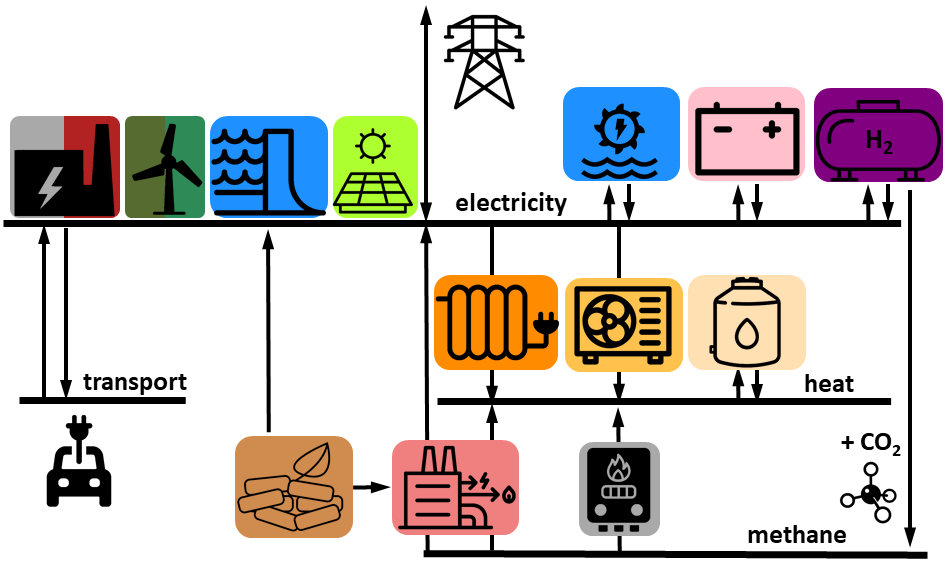
\includegraphics[width=\columnwidth]{../figures/model.png}
\caption{Model diagram representing the main generation and storage technologies in every country.} \label{fig_model} 
\end{figure}

\section{Data availability and code availability}

The model is implemented in the open-source framework Python for Power System Analysis (PyPSA) \cite{PyPSA}. The model and data used in this paper can be retrieved from \textcolor[rgb]{1,0,0}{XXX}

\section{Authors contribution}

M. Victoria designed the analysis, drafted the manuscript and contributed to the data acquisition, analysis and interpretation of data. K. Zhu contributed to the data acquisition, modelling, analysis and interpretation of data. 
T. Brown, G. B. Andresen and M. Greiner contributed to the initial idea and made substantial revisions of the manuscript. 

\section{Acknowledgements}
M. Victoria, K. Zhu, G. B. Andresen and M. Greiner are fully or partially funded by the RE-INVEST project, which is supported by  the  Innovation  Fund  Denmark  under  grant  number  6154-00022B. T.B. acknowledges funding from the Helmholtz Association under grant no. VH-NG-1352. The responsibility for the contents lies solely with the authors.

%\section{References}
\bibliography{bib_transition}

\end{document}